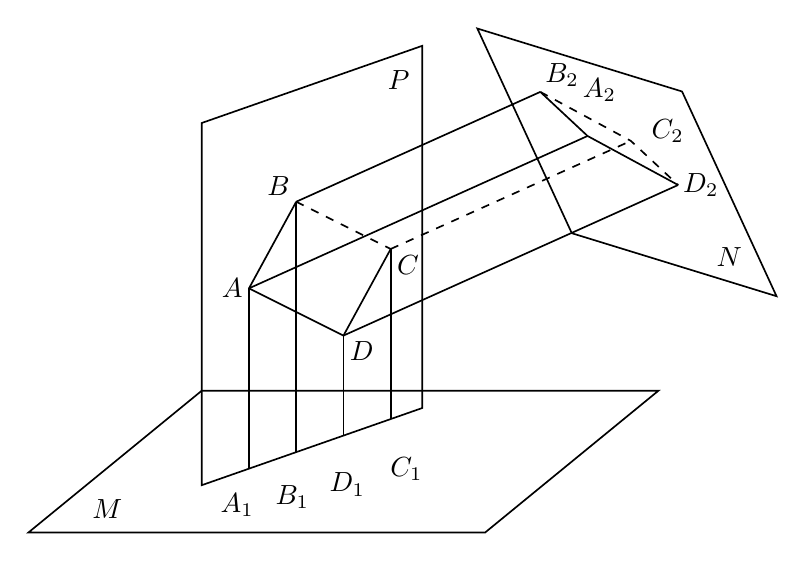
\begin{tikzpicture}[x=1cm,y=1cm,line width=.6pt,font=\normalsize]
\draw (0,-.6)--(5.8,-.6)--(8,1.2)--(2.2,1.2)--cycle;
\draw (2.2,0)--(5, .98)--(5,5.58)--(2.2,4.6)--cycle;
\draw (5.7,5.8)--(8.3,5)--(9.5,2.4)--(6.9,3.2)--cycle;
\coordinate (A) at (2.8,2.5);
\coordinate (B) at (3.4,3.6);
\coordinate (C) at (4.6,3);
\coordinate (D) at (4,1.9);
\coordinate (A1) at (2.8,0.21);
\coordinate (B1) at (3.4,0.42);
\coordinate (C1) at (4.6,0.84);
\coordinate (D1) at (4,0.63);
\coordinate (A2) at (7.1,4.435);
\coordinate (B2) at (6.5,4.995);
\coordinate (C2) at (7.65,4.3725);
\coordinate (D2) at (8.25,3.8125);
\draw (A)--(B);\draw[dashed] (B)--(C);\draw (C)--(D)--(A);
\foreach \p in {A,B,C,D}{\draw (\p)--(\p1);}
\draw (A)--(A2);\draw (B)--(B2);
\draw[dashed] (C)--(C2);\draw (D)--(D2);
\draw (A2)--(B2);\draw (A2)--(D2);\draw[dashed] (B2)--(C2)--(D2);
\node at (1,-.3) {$M$};\node at (4.7,5.15) {$P$};\node at (8.9,2.9) {$N$};
\node[left,inner sep=2pt] at (A) {$A$};
\node[above left,inner sep=2pt] at (B) {$B$};
\node[below right,inner sep=2pt] at (C) {$C$};
\node[below right,inner sep=2pt] at (D) {$D$};
\node[below,inner sep=1pt] at (2.65,-0.06) {$A_1$};
\node[below,inner sep=1pt] at (3.35,0.04) {$B_1$};
\node[below,inner sep=1pt] at (4.8,0.4) {$C_1$};
\node[below,inner sep=1pt] at (4.05,0.2) {$D_1$};
\node[inner sep=1.5pt] at (7.25,5.02) {$A_2$};
\node[above right,inner sep=1.5pt] at (B2) {$B_2$};
\node[right,inner sep=1.5pt] at (7.85,4.5) {$C_2$};
\node[right,inner sep=1.5pt] at (D2) {$D_2$};
\end{tikzpicture}
